
\subsection{ArcGIS produkty}

        V názvu práce se objevuje spojení Esri platforma, čímž jsou chápány
        produkty společnosti Esri. Esri je americká společnost zabývájící se
        vývojem software zaměřeného na geografické informační systémy. Manželé
        Dangermondovi ji založili v roce 1969\footnote{Více info
        http://www.esri.com/about-esri/history}.

        Z hlediska chápání Esri má GIS tři roviny. První je to GIS jako
        prostorová databáze reprezentující geografické informace, dále sada map
        zobrazující prvky a vztahy mezi prvky na zemském povrchu a zároveň i
        software pro GIS jako sada nástrojů pro odvozování nových informací ze
        stávajících. Esri tyto tři pohledy na GIS propojuje v software ArcGIS
        jakožto kompletní GIS, který se skládá z katalogu (kolekce geografický
        datových sad), map a sad nástrojů pro geografické analýzy.

        Esri vytváří integrovanou sadu softwarových produktů ArcGIS, které
        poskytují nástroje na kompletní správu GIS a přizpůsobují produkty
        různým úrovním nasazení. Výběr produktu záleží na tom, zda zákazník
        požaduje jedno nebo více uživatelský systém, zda se má jednat o stolní
        systém nebo server, popř. zda má být dostupný prostřednictvím
        internetu. Nabízí také produkty vhodné pro práci v terénu
        \citep{Esri2006}.

        Základními produkty\footnote{Názvy jednotlivých produktů použitých v
        tomto odstavci jsou platné od verze ArcGIS 10.1. Starší verze ArcGIS
        používají jiné názvy, jejichž přehled je možný na stránkách firmy ARCDATA
        Praha http://www.arcdata.cz/produkty-a-sluzby/software/arcgis/prejmenovani-arcgis/.
        } jsou stolní systémy ArcGIS for Desktop ve verzích Basic, Standard,
        Advanced\footnote{Zdroj http://www.esri.com/software/arcgis/about/gis-for-me},
        dále serverové verze ArcGIS for Server (pro Linux a Windows) ve třech úrovních
        funkcionality (Basic, Standard, Advanced) a dvou úrovních kapacity serveru
        (Workgroup a Enterpise). Další produkt ArcGIS for Mobile, ve verzích ArcPad,
        ArcGIS for Windows Mobile a ArcGIS for Smartphone and Tablet, je určený
        především pro práci v terénu. A v neposlední řadě verze dostupná skrze internet
        ArcGIS Online. K tomu všemu Esri přidává velké množství extenzí a další
        verzí\footnote{ Kompletní seznam na oficiálních webových stránkách Esri
        http://www.esri.com/products nebo http://www.arcdata.cz/produkty-a-sluzby/software/arcgis/}. 

          \begin{figure}[H]
            \centering
            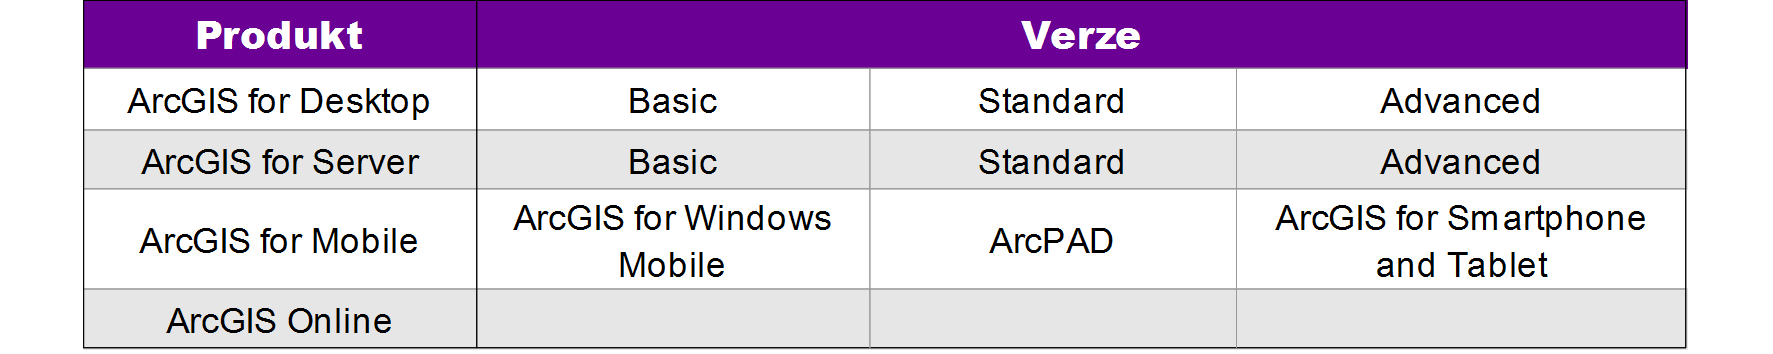
\includegraphics[width=1\textwidth]{../../../grafy/obr/tabulka_verzeArcGIS_primo.png}
            \caption{Verze programu ArcGIS platné od verze 10.1.}
          \end{figure}

        Dle \cite{Law2008} je nativním formátem produktů ArcGIS geodatabáze a
        jsou rozlišovány tři druhy geodatabáze. Ani v jednom případě se však
        nejedná o databázi v pravém slova smyslu, tak jako ji chápame v
        kapitole \odkazKapitola{PostgreSQL} a \odkazKapitola{MSSQL}. V každém případě však tyto způsoby umožňují
        uložení, přístup a správu dat. U prvních dvou typů, personální a
        souborové geodatabáze, se data ukládají do jednoho binárního souboru,
        kde jsou však ukládaná ve stejné struktuře jako v plnohodnotném
        databázovém serveru. Do takového geodatabáze můžeme uložit více než
        jednu vrstvu, což je výrazný rozdíl oproti formátu shapefile. Výhodou
        je dále možnost použití relací, sofistikované dotazování a v neposlední
        řadě i snadná přenostitelnost, protože takováto databáze bude vždy jen
        jeden soubor obsahující několik vrstev. Oproti tomu shapefile, který
        obsahuje jen jednu vrstvu, je tvořen minimálně 4 soubory. Oba tyto typy
        podporují pouze jednoho editujícího uživatele a mnoho uživetelů s
        právem čtení. Nepodporují dlouhé transakce ani verzování. 


          \begin{figure}[H]
            \centering
            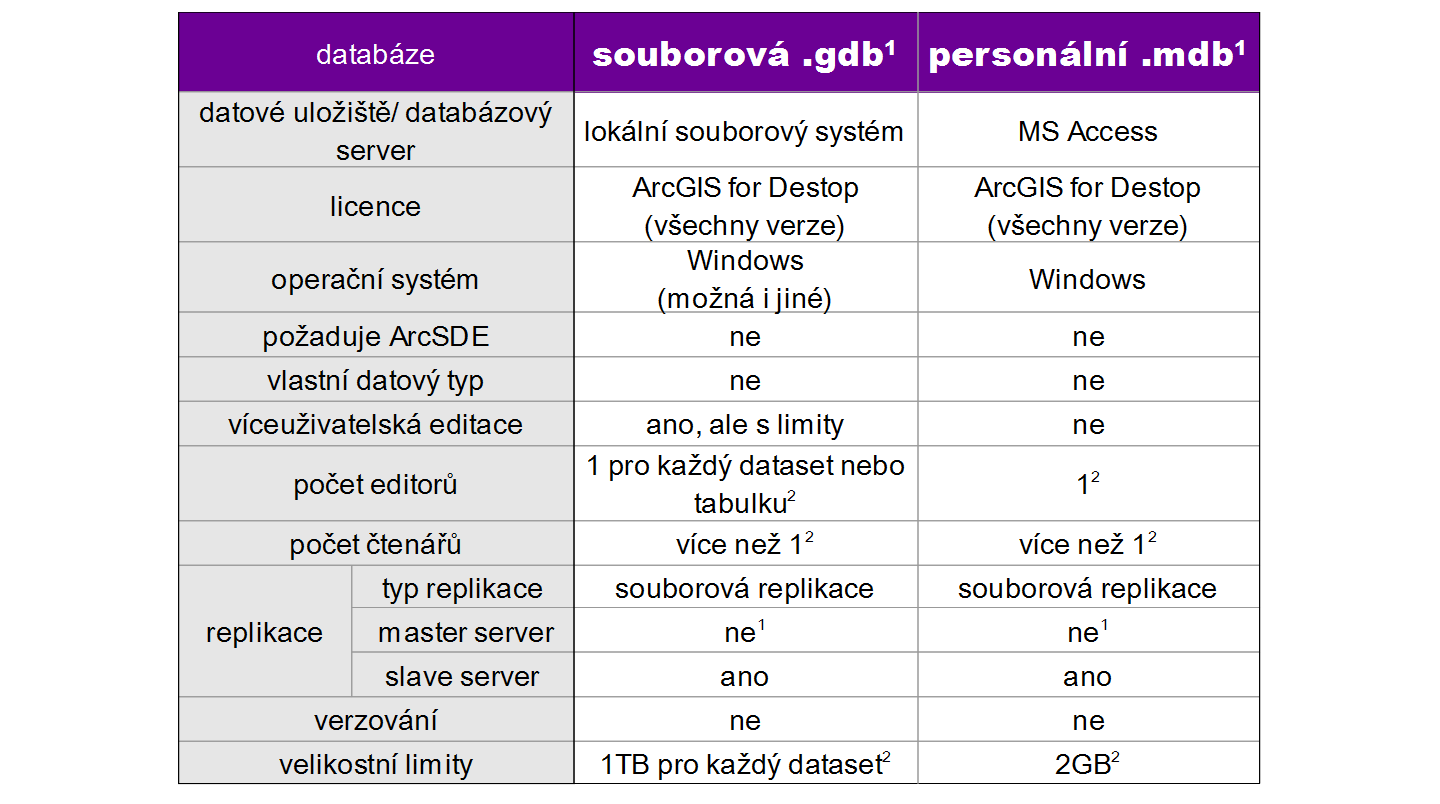
\includegraphics[width=1\textwidth]{../../../grafy/obr/tabulka_filePersonalDB_primo.png}
            \caption[Přehled rozdílů personální a souborové geodatabáze v ArcGIS]{Přehled rozdílů personální a souborové geodatabáze používané programem ArcGIS\newline\newline\textsuperscript{1}\small{http://www.esri.com/software/arcgis/geodatabase/single-user-geodatabase}\newline\textsuperscript{2}\small{http://help.arcgis.com/en/arcgisdesktop/10.0/help/index.html\#//003n00000007000000}
      }
          \end{figure}

        Tato práce se více zaměřuje na třetí typ, technologii ArcSDE, kterou v
        některých materiálech nazývají “geodatabáze ArcSDE”. Nejedná se o
        geodatabázi, ale spíše o zprostředkovatele komunikace mezi programem
        ArcGIS a databázovým server. Umožňuje víceuživatelský přístup,
        verzování i replikaci \citep{Esri2006}. Tato technologie využívá jako
        datové uložiště některý z již existujících databázových serverů, např.
        níže popsané PostgreSQL nebo MS SQL server. Touto technologií se více
        bude zabývat kapitola \odkazKapitola{ArcSDE} ArcSDE geodatabase.
